\documentclass[]{article}
\usepackage{graphicx}
\usepackage{hyperref}
\usepackage{amsmath}
\usepackage{caption}
\usepackage{subcaption}
\usepackage{float}

%opening
\title{Energy Gap in GaAs and Si}
\author{Gunther T\"urk, Jonas Lehnen}

\begin{document}

\maketitle
\begin{abstract}
In this experiment we want to measure the energy gaps for the semiconductors silicon Si and gallium arsenide GaAs. Thereby we want to see the difference between direct and indirect band transfer. To achieve appropriate values, calibration of photo diode and wavelength values have to be done in advance. In between the measurments for different temperatures the lamp spectrum has to be monitored to react to changes in our data caused by the room temperature. In the end we want to calculate values for the energy gaps and see how the absorption of photons differentiates between the different types of transfer.

\end{abstract}

\tableofcontents

\newpage
\section{Theory}
\subsection{Crystallography}
There are different types of crystals, depending on their inner structure, classified into the following groups. 

For the usual crystal structure, also called mono-crystal, the atoms are arranged evenly in a lattice as shown in figure \ref{fig:crystal structure}. Every atom has its specific place and the distance between them is always the same. The classical example would be the structure of carbon in a diamond, but also semi-conductors without doping are arranged in this way. The reason is the same amount of valence electrons. For Si and GaAs this distance, the lattice constant, is around $55nm$.

The polycrystalline structure is nearly the same as the mono-crystal. The difference is that the connection between some atoms is broken. This results in many crystals without regularity of shape and orientation. The same process can happen for a high concentration of colloids in a liquid. They can form poly-crystal like structures inside the medium they are floating in. Depending on temperature and mechanical forces, like shaking the sample, it is possible to see the crystals move in the liquid.

\begin{figure}[H]
\centering
\begin{subfigure}[h]{0.59\textwidth}
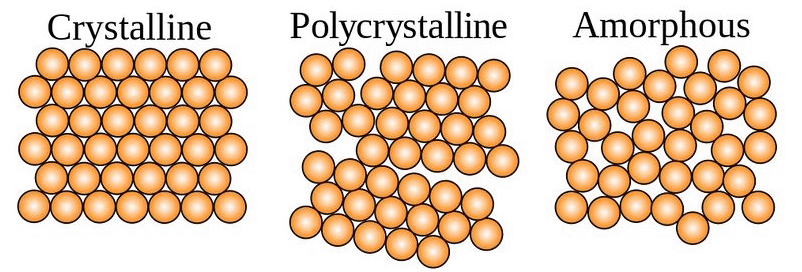
\includegraphics[width=1\textwidth]{Plots/crystalline.png}
\end{subfigure}
\begin{subfigure}[h]{0.39\textwidth}
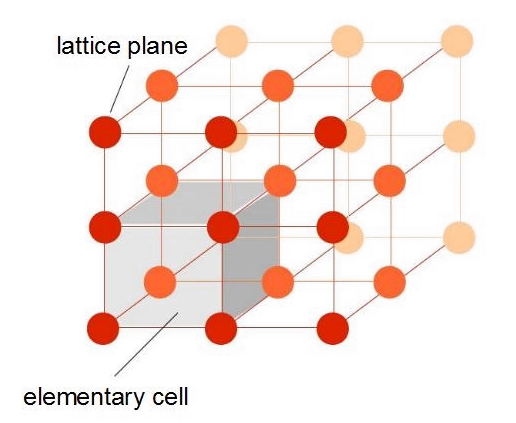
\includegraphics[width=1\textwidth]{Plots/lattice.png}
\end{subfigure}
\caption{Visualization of different solid states in the left. Lattice structure of a perfect crystal on the right. \cite{wiki}}
\label{fig:crystal structure}
\end{figure}

%%%%% vll ist colloids ein schlechts bsp, da es kein sollid ist

The last class are the amorphous solid bodies. In this state there is no structure in how the atoms in the crystal are arranged. Most of the man-made solid bodies are considered amorphous. For example glass, polymers and thin films created by sputtering. 

\subsection{Band structure}
  The band structure is derived from the Fermi-Dirac distribution. For fermions, spin=1/2 particles, there is a finite amount of how many of them are allowed to be in the same energy level. This is a result from Pauli's exclusion principle, where it's not possible to have 2 fermions with the exact same wave function. At a temperature $T=0K$ the electrons energy has to be the lowest possible. And thereby all states underneath the Fermi energy $E_F$ are occupied. There will be one spin up and down electron in each different energy level. For higher thermal energy the electrons can be excited to higher states and thereby the distribution flattens. The probability for electrons with higher energy than $E_F$ is increased.

\begin{figure}[H]
\centering
\begin{subfigure}[b]{1\textwidth}
	\centering
	\begin{equation}
	Fermi-Dirac \ statistics: \:\: W(E) = \frac{1}{exp\left(\frac{E-E_F}{k_B T}\right)+1} 
	\end{equation}
\end{subfigure}
\begin{subfigure}[b]{1\textwidth}
	\centering
	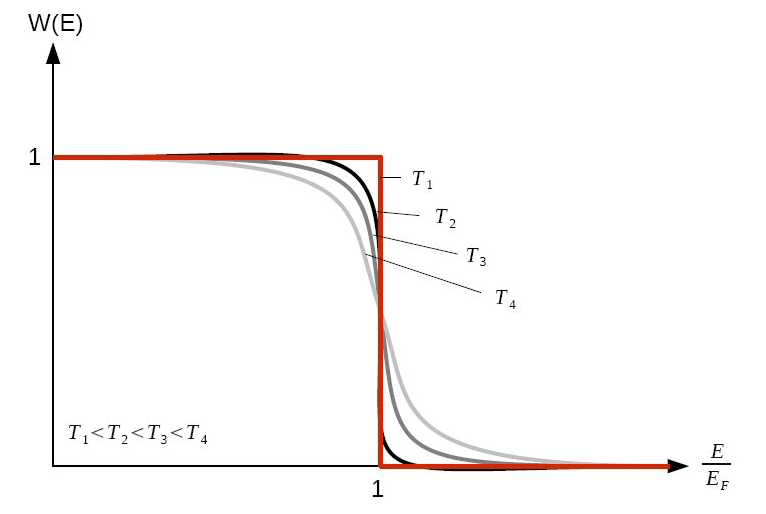
\includegraphics[width=.7\textwidth]{Plots/fd.png}
\end{subfigure}
\caption{Fermi-Dirac statistics equation on top and plots for different temperatures underneath, while $T_1=0K$. \cite{wiki}}
\end{figure}

Considering many Coulomb potentials in a one-dimensional lattice, their energy levels overlap and shift each other apart. This happens if they are in the same state, due to Pauli and the electromagnetic interaction between the electrons. The shifted discrete levels are still close to each other and can be summarized into a band with a thickness regarding to the energy. The first band in which the electrons are no longer bound to a nucleus is called the conduction band. If an electron has such a high energy it can be used for a current through the solid. The last band in which the electrons are still bound is called valence band. This means that their energy is not enough to leave the potential, but they are able to change the nucleus by tunneling. This causes no current, because the probability for tunneling into another potential is as low as the reversed way. The average effect is thereby zero.

There are 3 types of solids, regarding their distance between valence and conduction band. This distance is called energy gap. There is no gap in metal solids. Electrons are free to be used as current and can change their nucleus. Insulators are the opposite. Their energy gap is extremely high, around $5eV$. This means a high voltage is necessary to excite them into the conduction band. Usually the high voltage would break the insulator, due to power in the form of heat. A semi-conductors energy gap is around $1eV$. This means it is possible to excite them by applying a voltage and thereby creating conductivity.

\begin{figure}[H]
\centering
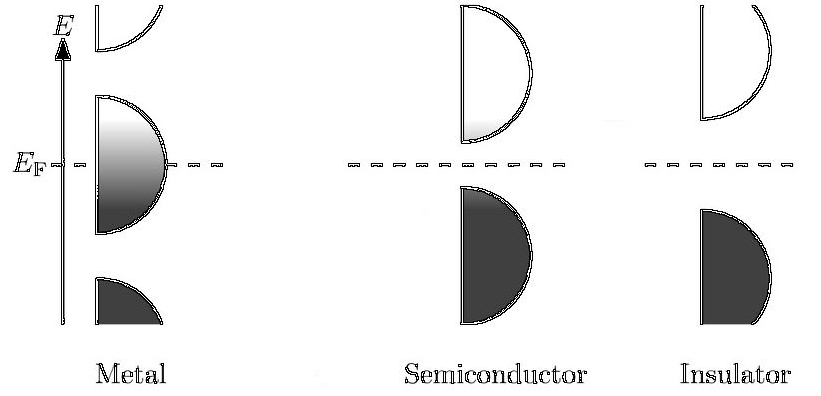
\includegraphics[width=.7\textwidth]{Plots/bandstructure.png}
\caption{Schematic illustration of different types of metal. White: conduction band. Black: valence band. Difference between the bands is equal to the energy gap. The Fermi energy is exactly between the both bands energy. \cite{wiki}}
\label{fig:bandstructure}
\end{figure}

Besides a dependency on temperature, the energy gap can change in the process of doping. This considers adding different atoms into a semi-conducting material. Most of the time atoms with three or five valence electrons are used. This results in p- and n-doped versions of the semi-conductor. In the band structure of a n-doped semi-conductor an additional energy level is created underneath the conduction band, due to an additional valence electron which has no partner to form a covalent bond. This electron is only bond to its nucleus and therefore easily excitable with less energy.
In the p-doped version another energy level above the valence band is created. A missing electron for a covalent bond can be replaced by one of the lattice forming ones. Form the foreign atom the electron can be easily excited, due to less binding energy. This means a electron can take two steps, each with lesser energy than the energy gap, to become excited into the conduction band.

\subsection{Band transfer}
For temperatures $T\neq 0$ atoms are oscillating due to their thermal energy. It is possible to quantize this energy analogue to a photons energy. Those analogue particles of the lattice oscillations are called phonons. Just like the photons they are described by momentum $\hbar K$ and energy $\hbar \Omega_K$. This energy has to be considered while calculating the energy gap, due to different types of band transfer.

The obvious direct band transfer is not depending on any phononic influence. Maximum of valence and minimum of conduction band are at the same wave vector. This means the excitation happens without a change of momentum. Therefore only a photon, which can't change the crystals momentum, in necessary to deliver the transition energy.

\begin{figure}[H]
\centering
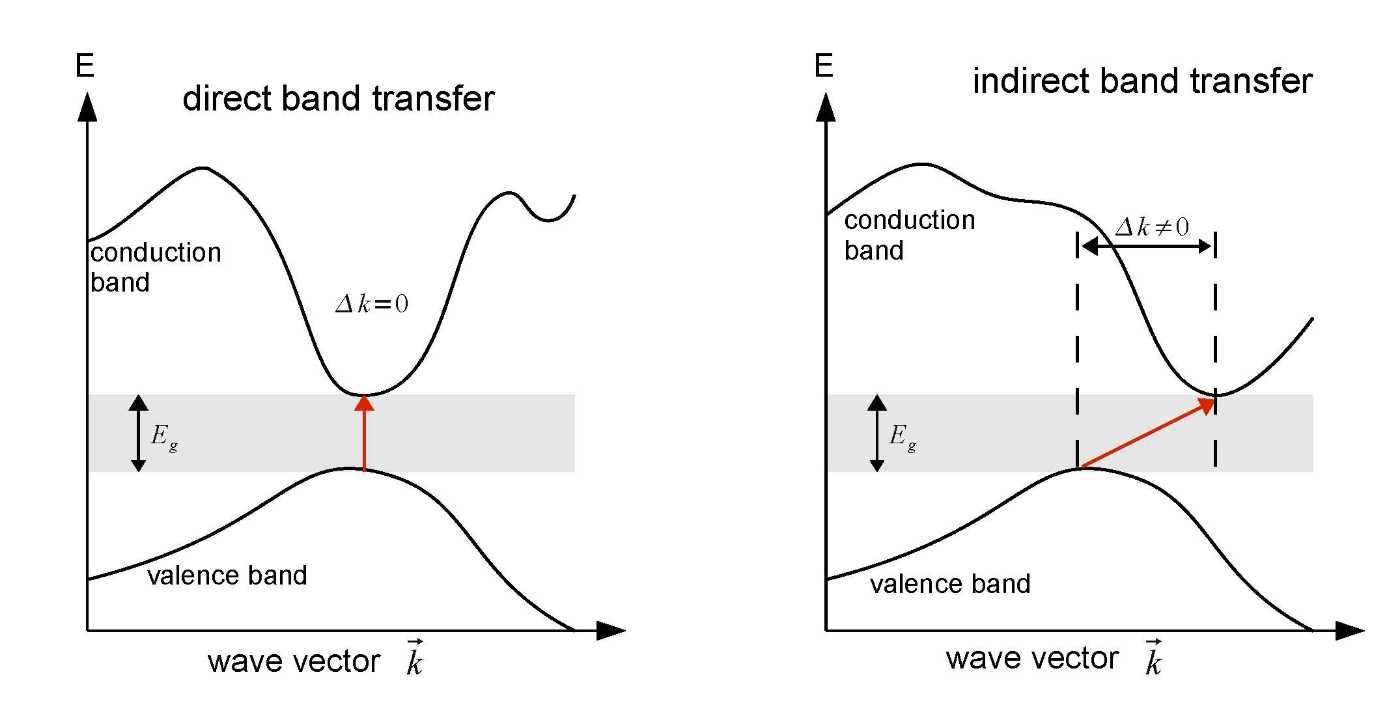
\includegraphics[width=.8\textwidth]{Plots/transfer.png}
\caption{Illustration of direct and indirect band transfer. \cite{wiki}}
\label{fig:band transfer}
\end{figure}

In materials with an indirect band gap, e.g. silicon, the valence maxima and conduction minima are not at the same momentum of the atoms electron. In this case the transition energy is still delivered by the photon, but a change in the lattice momentum is necessary. This happens by emitting or absorbing a phonon, because photons can't change the oscillation of the crystal in such a scale. The probability of excitation into the conduction band is less than in the direct transfer. Reason behind this is the necessary temperature, without it no phonons could exist. The phonons energy is very low. For example $T=500K$: $ E_P= \hbar \Omega_K = kT = 0.043 eV$.
There are two possibilities how the excitation can happen. If the photons energy is less than the energy gap, a existing phonon has to be absorbed. If the energy is higher than necessary, a phonon gets emitted. 

Light Emitting Diodes are usually produced from materials with a direct band gap. In this way the intensity of light emitted is higher and more consistent.

\subsection{Lambert-Beer law}
The Lambert-Beer law describes the relation between absorbed light passing through a solid material, depending on its thickness $dx$ and the materials absorption coefficient $\alpha$. This coefficient also describes the   product of photon absorbing centres per volume $N$ and their effective cross section $\sigma$ to absorb. 

\begin{equation}
\label{eq:Lambert-Beer}
-dI(x) = \alpha \cdot I(x)\cdot dx\ \rightarrow\ \alpha=\frac{ln(I_0 / I(x))}{x} = N\cdot \sigma
\end{equation}

To determine the indirect energy gap of silicon the absorption coefficient is approximated with the following equation. In this case the photons energy $h\nu$, the energy gap $E_g$ and the phonons energy $E_p$ are variable as well as the temperature $T$.

\begin{equation}
\alpha \propto  \frac{(h\nu - E_g + E_p)^2}{exp\left(\frac{E_p}{kT}\right) -1} + \frac{(h\nu - E_g - E_p)^2}{1-exp\left(\frac{E_p}{kT}\right)} 
\end{equation}


\section{Experiment}
\subsection{Set-up}
Via a monochromator only light of a certain wavelength can be filtered. This wavelength will later determine the energy of the light. By turning a screw on the monochromator the reflection lattice turns and the scale should display the wavelength which is passing through the monochromator. If the lights energy is sufficient the semiconductor will be able to absorb it and in there will be no intensity noticeable at our photo diode. 

\begin{figure}[H]
\centering
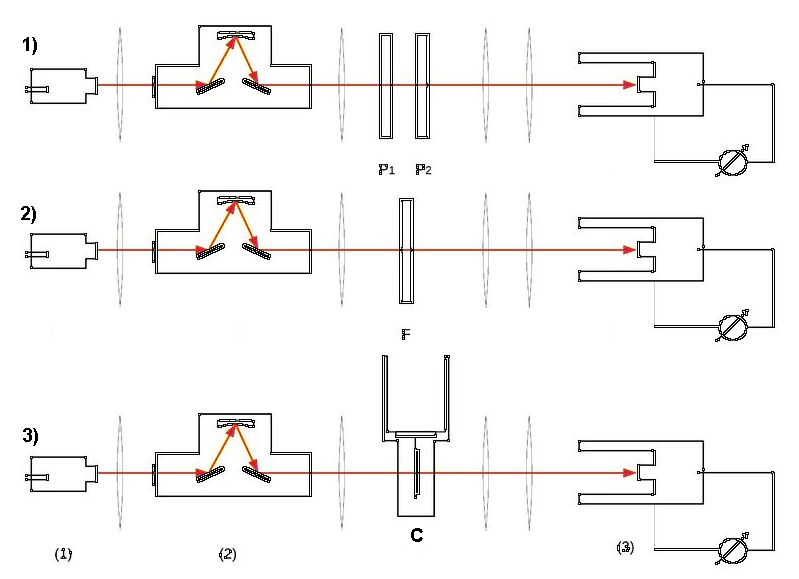
\includegraphics[width=.9\textwidth]{Plots/setup.png}
\caption{Set-up for this experiment. (1) Lamp, (2) Monochromator, (3) Photo diode, C Cryostat, P1/P2 Polarisation filter, F Coloured filter. }
\label{fig:setup}
\end{figure}

There are four different set-ups used in this experiment. All of them are consisting of a lamp (1), a monochromator (2) and a photo diode (3) arranged as always shown in figure \ref{fig:setup}. In between the part, lenses are placed to keep a focused light path.

1: In the first task the polarisation filters P1/P2 were placed as shown. We aligned the polarisation axis of both filters and then started turning the rear filter. We measured the light current of the diode for several angles $\alpha$ between $0^\circ$ and $90^\circ$. Thereby we want to show that with linear increase in light intensity, the photo-current increases linearly, too. %This ensures that the photo diode registers all of the incoming light.
If the diode is linear, the measured intensities only differ by a constant factor from the actual light intensity. This factor can be neglected because it will be fitted by an arbitrary coefficient in any case.

2: Task two consists of calibrating our monochromator by measuring the intensity while coloured filters F are in the lights path. With this we will compare the values given on the monochromator to the Gaussian peaks in the intensity. This leads to a correction function and more precise wavelengths to calculate the energy gaps.

3: The third set-up includes the cryostat C with included samples of Si and GaAs. Taking a full lamp spectrum from $400nm \ - \ 1200nm$ we can then see where the photo diode starts measuring light again. This energy will be equivalent to the gap. Each measurement will be performed twice. Once with the samples at room temperature and once with them cooled to  $T=77K$ with liquid nitrogen.

Before the normal temperature measurement, in between normal and cold measurement and at the end an additional lamp spectra are taken. This happens without any of the third components in figure \ref{fig:setup}. Thereby we want to observe if the conditions of the different energy gap measurements are constant and where to expect to see the photo-current. 


\subsection{Photo diode}
The light intensity is proportional to the square of the light amplitude. Behind the second polarisation filter we should measure the intensity:
\begin{equation}
	I \propto sin(\alpha)^2
\end{equation}
To show that the photo current scales linearly with the light intensity we plotted $\frac{I}{I_{\alpha=0}}$ against $sin(\alpha)^2$ and found a linear correlation with a gradient of -1. So we have a direct proportionality between our photo current and the light intensity.

\subsection{Coloured filters} \label{color filters}
Now we want to see if the values the monochromator screw displays us are the same wavelengths the coloured filters are supposed to pass. Supposing the filters information about the wavelength is more reliable than a screw with mechanical settings, we will calibrate them accordingly.

For the given values on the filters we checked 30 surrounding wavelengths for each filter to find each maximums intensity. The Gaussian fits were made with the function:
\begin{equation}
f(x) = A \cdot e^{-\frac{(x-\mu)^2}{2 \sigma^2}} + b
\end{equation}

\begin{figure}[H]
\centering
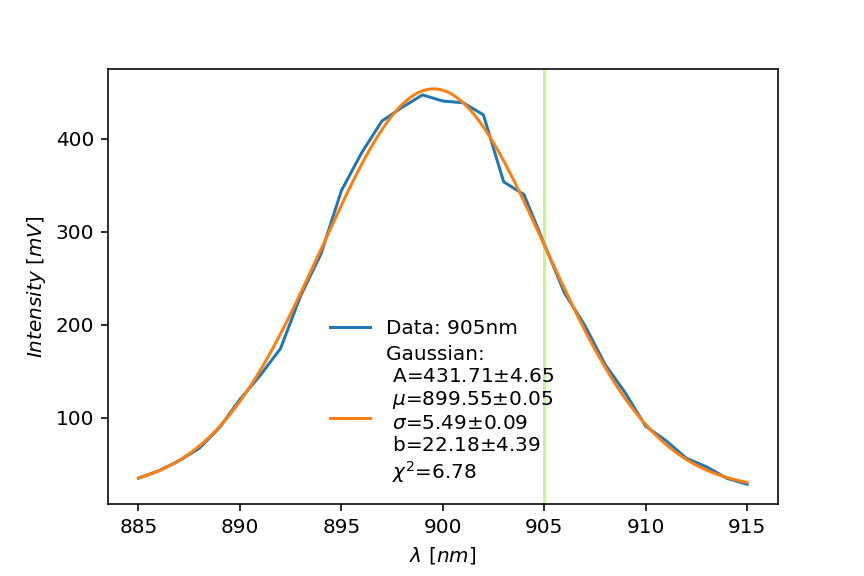
\includegraphics[width=.9\textwidth]{Plots/905nm-Filter.png}
\caption{Fit for the wavelength calibration at 905nm. Green line indicates the value given on the filters. The other filters are shown in Chapter \ref{Appendix} Appendix, as well as the raw data.}
\end{figure}

\begin{table}[H]
	\centering
	\begin{tabular}{c|c|c|c}
	Filter [nm] & 768 & 905 & 1060 \\ \hline
	Fit [nm] & 764.92(6) & 899.55(5) & 1071.10(13) \\ \hline
	Difference [nm] & -3.08 & -5.45 & 11.10
	\end{tabular}
	\caption{Comparison of expected and measured maximum intensity wavelength. The filter value is the more trustful to be correct.}
\end{table}

We can now determine how we have to change the wavelengths for the following measurements, by interpolating the values with a straight line:

\begin{figure}[H]
\centering
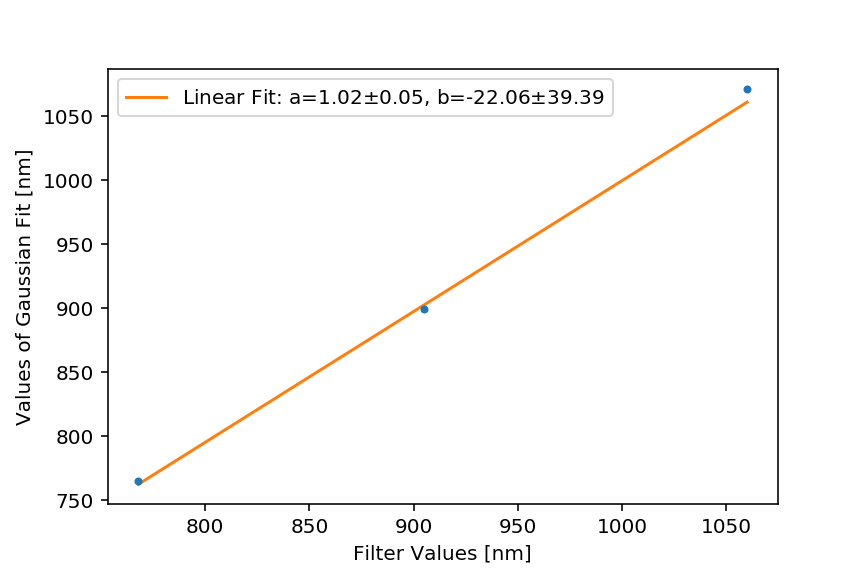
\includegraphics[width=.9\textwidth]{Plots/LambdaCorrection.png}
\caption{Correction of the monochromator values, due to the measurements with the coloured filters.}
\label{fig:LambdaCorrection}
\end{figure}

For the calculation of the energy gaps, we now have to consider changing the measured values to correct the difference between filters and monochromator. This follows the linear equation used for the fit: 
\begin{equation}
\lambda_{real} = a\cdot \lambda_{measured} \ + \ b
\end{equation}

\subsection{Lamp spectrum} \label{lamp spectrum}
In the case of changes relating to the light of our lamp during the time of the experiment, we took the whole lamp spectrum before the first, in between and after the second measurement with the semiconductors in the lights path. It is possible, due to changes in temperature, that the intensities could fluctuate. This would affect the determination of the energy gap. If the plateau area is decreased, the edge of the spectrum could be broader. For the sample on the right of the cryostat, this could increase the difficulty to determine a specific wavelength.

But in our case nothing like this happened, as shown in figure \ref{fig:lamp spectra}, where the wavelengths are not yet calibrated with the $2\%$ from section \ref{color filters}.

\begin{figure}[H]
\centering
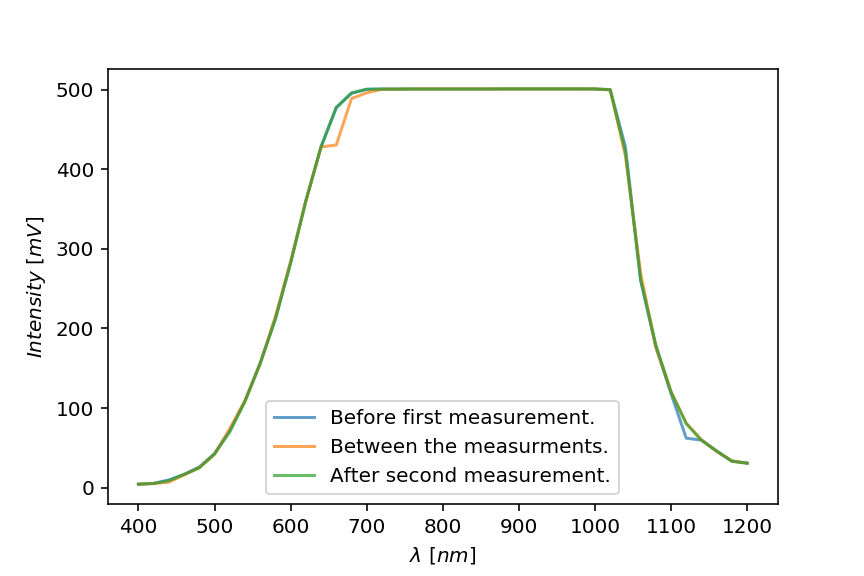
\includegraphics[width=.8\textwidth]{Plots/All-Lamp-Spectra.png}
\caption{All three measurements of the whole lamp spectrum. The measurements in the legend is related to the following measurements of the energy gaps at different temperatures.}
\label{fig:lamp spectra}
\end{figure} 

As you can see the intensities are dropping rapidly after  $\lambda =1000nm$, for each spectrum. Except of some divergences, which could be caused by rapidly changing the wavelength, they are nearly the identical. The exact measured values are shown in Chapter \ref{Appendix} Appendix.

This concludes in constant conditions for the energy gap measurements for silicon an gallium arsenide in the next chapter.

\subsection{Energy Gaps}
We had GaAs and Si as our samples but did not know which one was which. So to figure that out, we plotted the raw data (\ref{fig:raw-data}) and immediately saw two different types of energy gaps. For the two curves of GaAs we see a sharp edge where the intensity drops to zero between $800$ and $900nm$. This fits well with the literature value of the GaAs energy gap of $1.45eV$ and shows, that there are not many other factors influencing the energy gap like phonons. In case of the silicon we see a much smoother edge, because phonons can cause absorption before the photons have the energy of the gap.
\subsubsection{GaAs (direct gap)}
To find the energy gap of GaAs we fitted the sudden decrease in intensity and the long slope behind it linear with two different fits. The intersection should then give us the Energy gap. This gave us an energy of $892.8nm$ or around $1.39eV$ at 300K and $847nm$ or $1.46eV$ at 77K. As expected the energy of the band gap is slightly larger (around $5\%$) at a very low temperature cause we lower the energy of phonons which can effectively make the bang gap smaller. 

\subsubsection{Silicon (indirect gap)}
For the indirect gap we needed to fit the absorption coefficient (\ref{eq:Lambert-Beer}) with the approximation
\begin{equation}
\label{fit function}
\alpha = A\cdot \left[ \frac{(h\nu - E_g + E_p)^2}{exp\left(\frac{E_p}{kT}\right) -1} + \frac{(h\nu - E_g - E_p)^2}{1-exp\left(\frac{E_p}{kT}\right)} \right]
\end{equation}
where $E_g$ is the Energy of the gap and $E_p$ is the phonon energy.


This formula is valid only for light with photon energy larger, but not too much larger, than the band gap (more specifically, this formula assumes the bands are approximately parabolic), and ignores all other sources of absorption other than the band-to-band absorption in question, as well as the electrical attraction between the newly created electron and hole (see exciton). It is also invalid in the case that the direct transition is forbidden, or in the case that many of the valence band states are empty or conduction band states are full.\cite{absformular}
For actually fitting the data we tried to use only values larger than the energy gap and only accepted fits, where the photon energy was larger than the phonon energy. This gave us $0.80eV$ at 300K and $1.20eV$ at 77K
%Prozentualer vgl und sagen warum der hier so viel größer ist.


\begin{figure}
	\centering
	\includegraphics[width=0.7\linewidth]{"Plots/raw data"}
	\caption{}
	\label{fig:raw-data}
\end{figure}





%%% Thickness of sample -> constant and absorbed in A in the  fit eqzuation
%%% Gutnher: Jo nehme ich mal schwer an xD
\subsection{Conclusion} \label{Conclusion}
In the end we want to talk about error sources. As shown in chapter \ref{lamp spectrum} the spectrum seemed to be constant as well as the room temperature. The position if the cryostat wasn't the same for different temperatures. This could affect the thickness of the sample, but we tried to position it vertical to the lights path. 

In the script it was mentioned to take care of nitrogen clouds and condensation at the cryostats window. These effects could cause decreased intensities measured by the photo diode. By covering the nitrogen with aluminium foil and heating the windows, their influence should be minimized and not noticeable.

In section \ref{color filters} it was strange that the $1060nm$ filter show a displacement to the left instead of the right like the other. The reason for this result seems to be the rapidly dropping intensity after the $\lambda =1000nm$, as discussed in section \ref{lamp spectrum}. After all only 3 filters to calibrate the wavelength seems to be insufficient for excellent results.

The worst error source is the monochromator screw. Although the scale should be correct, the measurements with the filters corrected it. The display of the scale itself seemed to be uncertain on $0.5nm$, because it was possible to turn the screw for a bit without changing the number displayed on the scale. 


\newpage
\section{Appendix} \label{Appendix}
\begin{figure}[H]
\centering
\begin{subfigure}[b]{0.9\textwidth}
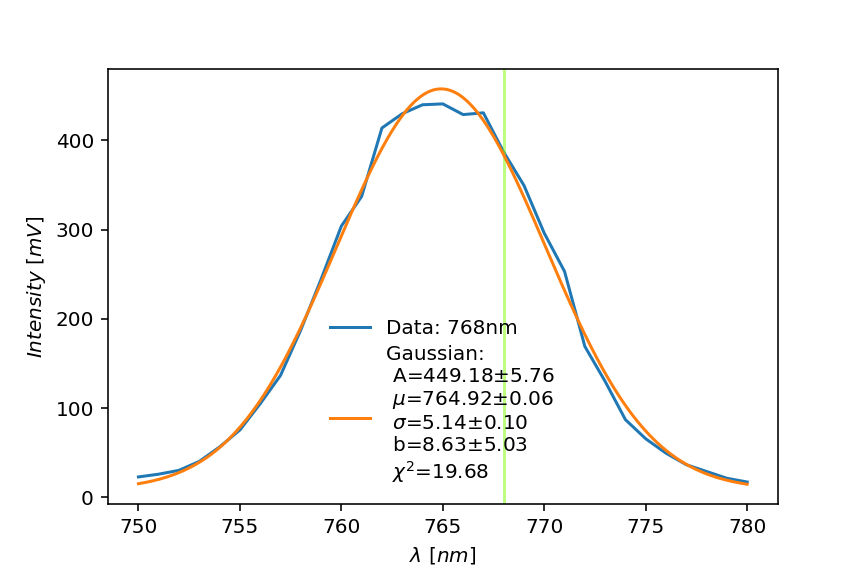
\includegraphics[width=\textwidth]{Plots/768nm-Filter.png}
\end{subfigure}
\begin{subfigure}[b]{0.9\textwidth}
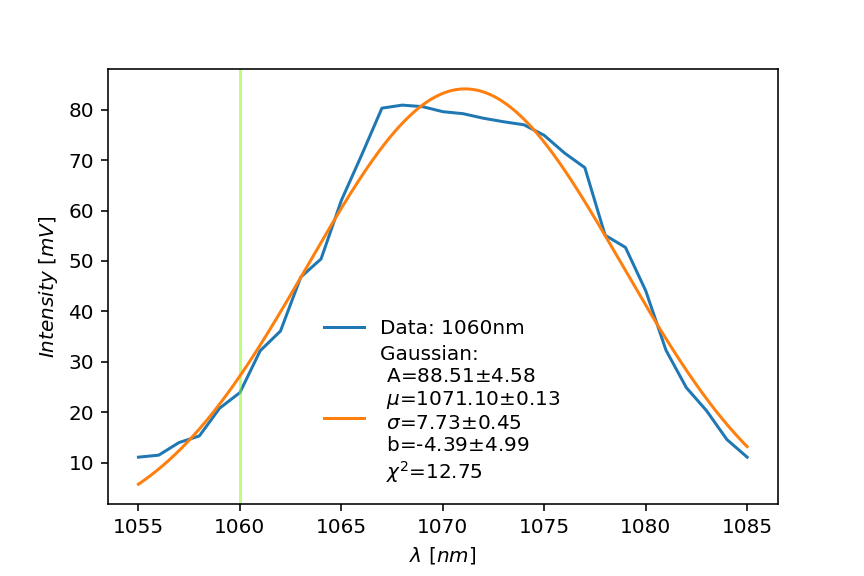
\includegraphics[width=\textwidth]{Plots/1060nm-Filter.png}
\end{subfigure}
\caption{Other filter calibrations from section \ref{color filters}. }
\end{figure}

\begin{table}[H]
\centering
\begin{tabular}{|c|c||c|c||c|c|}
\hline
$\lambda$ 1 [nm] & I 1 [mV] & $\lambda$ 2 [nm] & I 2 [mV] & $\lambda$ 3 [nm] & I 3 [mV] \\ \hline\hline
400.0 & 4.4 & 400.0 & 4.3 & 400.0 & 4.3 \\ \hline
420.0 & 5.4 & 420.0 & 5.2 & 420.0 & 5.2 \\ \hline
440.0 & 9.7 & 440.0 & 6.9 & 440.0 & 8.7 \\ \hline
460.0 & 16.7 & 460.0 & 16.0 & 460.0 & 16.6 \\ \hline
480.0 & 26.1 & 480.0 & 25.1 & 480.0 & 24.8 \\ \hline
500.0 & 42.8 & 500.0 & 41.9 & 500.0 & 42.3 \\ \hline
520.0 & 72.1 & 520.0 & 73.8 & 520.0 & 69.8 \\ \hline
540.0 & 109.0 & 540.0 & 109.4 & 540.0 & 108.0 \\ \hline
560.0 & 156.7 & 560.0 & 155.7 & 560.0 & 155.7 \\ \hline
580.0 & 212.0 & 580.0 & 215.1 & 580.0 & 212.0 \\ \hline
600.0 & 283.1 & 600.0 & 284.0 & 600.0 & 281.8 \\ \hline
620.0 & 360.4 & 620.0 & 360.0 & 620.0 & 360.0 \\ \hline
640.0 & 428.3 & 640.0 & 428.0 & 640.0 & 428.0 \\ \hline
660.0 & 477.3 & 660.0 & 430.4 & 660.0 & 477.6 \\ \hline
680.0 & 495.3 & 680.0 & 488.7 & 680.0 & 495.9 \\ \hline
700.0 & 500.3 & 700.0 & 495.9 & 700.0 & 500.5 \\ \hline
720.0 & 500.7 & 720.0 & 500.4 & 720.0 & 500.7 \\ \hline
740.0 & 500.6 & 740.0 & 500.5 & 740.0 & 500.7 \\ \hline
760.0 & 500.7 & 760.0 & 500.8 & 760.0 & 500.8 \\ \hline
780.0 & 500.7 & 780.0 & 500.8 & 780.0 & 500.8 \\ \hline
800.0 & 500.7 & 800.0 & 500.8 & 800.0 & 500.8 \\ \hline
820.0 & 500.7 & 820.0 & 500.8 & 820.0 & 500.8 \\ \hline
840.0 & 500.7 & 840.0 & 500.8 & 840.0 & 500.8 \\ \hline
860.0 & 500.7 & 860.0 & 500.8 & 860.0 & 500.8 \\ \hline
880.0 & 500.8 & 880.0 & 500.8 & 880.0 & 500.9 \\ \hline
900.0 & 500.8 & 900.0 & 500.8 & 900.0 & 500.9 \\ \hline
920.0 & 500.8 & 920.0 & 500.8 & 920.0 & 500.9 \\ \hline
940.0 & 500.8 & 940.0 & 500.8 & 940.0 & 500.9 \\ \hline
960.0 & 500.8 & 960.0 & 500.8 & 960.0 & 500.9 \\ \hline
980.0 & 500.8 & 980.0 & 500.8 & 980.0 & 500.9 \\ \hline
1000.0 & 500.8 & 1000.0 & 500.8 & 1000.0 & 500.8 \\ \hline
1020.0 & 500.0 & 1020.0 & 499.7 & 1020.0 & 499.7 \\ \hline
1040.0 & 428.0 & 1040.0 & 416.6 & 1040.0 & 421.3 \\ \hline
1060.0 & 260.4 & 1060.0 & 269.4 & 1060.0 & 261.3 \\ \hline
1080.0 & 176.6 & 1080.0 & 176.4 & 1080.0 & 179.4 \\ \hline
1100.0 & 117.9 & 1100.0 & 120.6 & 1100.0 & 120.2 \\ \hline
1120.0 & 62.1 & 1120.0 & 81.0 & 1120.0 & 80.3 \\ \hline
1140.0 & 59.8 & 1140.0 & 60.0 & 1140.0 & 59.4 \\ \hline
1160.0 & 45.5 & 1160.0 & 45.6 & 1160.0 & 46.2 \\ \hline
1180.0 & 33.5 & 1180.0 & 33.5 & 1180.0 & 33.0 \\ \hline
1200.0 & 30.8 & 1200.0 & 30.9 & 1200.0 & 30.6 \\ \hline
\hline
\end{tabular}
\caption{Data for the lamp spectrum plots. Before:1, Between:2, After:3. }
\end{table}

\begin{table}[H]
\centering
\begin{tabular}{|c|c||c|c||c|c|}
\hline
768: $\lambda$ [nm] & I [mV] & 905: $\lambda$ [nm] & I [mV] & 1060: $\lambda$ [nm] & I [mV] \\ \hline\hline
750.0 & 22.9 & 885.0 & 35.0 & 1055.0 & 11.1 \\ \hline
751.0 & 26.0 & 886.0 & 43.0 & 1056.0 & 11.5 \\ \hline
752.0 & 30.3 & 887.0 & 53.7 & 1057.0 & 14.0 \\ \hline
753.0 & 40.3 & 888.0 & 67.2 & 1058.0 & 15.3 \\ \hline
754.0 & 56.5 & 889.0 & 89.5 & 1059.0 & 20.8 \\ \hline
755.0 & 75.5 & 890.0 & 119.7 & 1060.0 & 23.9 \\ \hline
756.0 & 104.9 & 891.0 & 145.6 & 1061.0 & 32.2 \\ \hline
757.0 & 136.6 & 892.0 & 174.4 & 1062.0 & 36.1 \\ \hline
758.0 & 187.5 & 893.0 & 231.6 & 1063.0 & 46.8 \\ \hline
759.0 & 244.4 & 894.0 & 276.5 & 1064.0 & 50.4 \\ \hline
760.0 & 304.0 & 895.0 & 344.3 & 1065.0 & 62.0 \\ \hline
761.0 & 337.3 & 896.0 & 385.1 & 1066.0 & 71.0 \\ \hline
762.0 & 414.0 & 897.0 & 419.3 & 1067.0 & 80.3 \\ \hline
763.0 & 430.0 & 898.0 & 434.1 & 1068.0 & 80.9 \\ \hline
764.0 & 440.0 & 899.0 & 447.4 & 1069.0 & 80.6 \\ \hline
765.0 & 441.0 & 900.0 & 440.8 & 1070.0 & 79.6 \\ \hline
766.0 & 429.0 & 901.0 & 439.0 & 1071.0 & 79.2 \\ \hline
767.0 & 431.0 & 902.0 & 426.0 & 1072.0 & 78.3 \\ \hline
768.0 & 387.0 & 903.0 & 353.8 & 1073.0 & 77.6 \\ \hline
769.0 & 349.6 & 904.0 & 340.2 & 1074.0 & 77.0 \\ \hline
770.0 & 296.1 & 905.0 & 287.0 & 1075.0 & 74.9 \\ \hline
771.0 & 253.2 & 906.0 & 234.1 & 1076.0 & 71.4 \\ \hline
772.0 & 169.2 & 907.0 & 199.3 & 1077.0 & 68.5 \\ \hline
773.0 & 130.0 & 908.0 & 157.3 & 1078.0 & 55.1 \\ \hline
774.0 & 87.1 & 909.0 & 126.6 & 1079.0 & 52.7 \\ \hline
775.0 & 65.7 & 910.0 & 90.8 & 1080.0 & 44.1 \\ \hline
776.0 & 49.5 & 911.0 & 75.4 & 1081.0 & 32.3 \\ \hline
777.0 & 36.6 & 912.0 & 56.5 & 1082.0 & 24.9 \\ \hline
778.0 & 29.0 & 913.0 & 47.2 & 1083.0 & 20.3 \\ \hline
779.0 & 21.4 & 914.0 & 34.9 & 1084.0 & 14.6 \\ \hline
780.0 & 17.2 & 915.0 & 28.5 & 1085.0 & 11.1 \\ \hline
\hline
\end{tabular}
\caption{Data values for the different coloured filter plots. The filters given wavelength [nm] is displayed upper left corner for each 2 rows. }
\end{table}
% Tabellen der ganzen dummen Werte


\newpage
\begin{thebibliography}{}

\bibitem{wiki} \begin{verbatim}
http://wiki-fp.physik.uni-mainz.de/index.php/44_energy_gap_in_GaAs_and_Si
\end{verbatim} 
\bibitem{absformular}
\begin{verbatim}
	3.^ Jump up to: a b J.I. Pankove, Optical Processes in Semiconductors. Dover, 1971
\end{verbatim}



\end{thebibliography}
\end{document}

